\documentclass{article}
\usepackage{amsmath, amsthm, amssymb, amsfonts, booktabs, hyperref, graphicx, float, esint, xcolor, subcaption, xspace}
\usepackage[margin=1.0in]{geometry}
% mathbbol, causing errors
\setlength{\abovedisplayskip}{0pt}
\setlength{\belowdisplayskip}{0pt}
\setlength{\abovedisplayshortskip}{0pt}
\setlength{\belowdisplayshortskip}{0pt}

\newcommand{\vr}{\vec{r}}
\newcommand{\vx}{\vec{x}}
\newcommand{\vOmega}{\vec{\Omega}}
\newcommand{\vJ}{\vec{J}}
\newcommand{\vp}{\vec{p}}
\newcommand{\vO}{\vec{\Omega}}
\newcommand{\bra}{\left\langle}
\newcommand{\ket}{\right\rangle}
\newcommand{\ketbd}{\right\rangle_{\delta \Omega}}
\newcommand{\sbra}{\left[}
\newcommand{\sket}{\right]}
\renewcommand{\div}{\vec{\nabla} \cdot}
\newcommand{\grad}{\vec{\nabla}}
\newcommand{\vbeta}{\vec{\beta} }
\newcommand{\pdx}{\frac{\partial}{\partial x}}
\newcommand{\pdy}{\frac{\partial}{\partial y}}
\newcommand{\pdz}{\frac{\partial}{\partial z}}
\newcommand{\intrrr}{\int d^3 r \,}
\newcommand{\intrr}{\int d^2 r \,}
\newcommand{\dEdphi}{\partial_\phi E }
\newcommand{\dEdp}{\partial_p E }
\newcommand{\dBdphi}{\partial_\phi B }
\newcommand{\dBdp}{B }
\newcommand{\adj}{\phi^\dag}
\newcommand{\surf}{\int_{\partial V}}
\newcommand{\domain}{V}
\newcommand{\bound}{\partial V}
\newcommand{\vn}{\vec{n}}
\newcommand{\Edd}{\mathbb{E}}
\newcommand{\BEdd}{B}
\newcommand{\sigt}{\sigma_t}
\newcommand{\sigs}{\sigma_s}
\newcommand{\siga}{\sigma_a}
\newcommand{\isigt}{c}
% why \newcommand{\angSource}{q_\Omega}
\newcommand{\angSource}{q}
\newcommand{\scalSource}{q}
\newcommand{\angResp}{q^\dag}
\newcommand{\scalResp}{q^\dag}
\newcommand{\qoi}{{\it QoI}\xspace}
\newcommand{\Ui}{U_i}
\newcommand{\Uipo}{U_{i+1}}
\newcommand{\Uimo}{U_{i-1}}
\newcommand{\Uo}{U_o}
\newcommand{\Uopo}{U_{o+1}}
\newcommand{\Uomo}{U_{o-1}}
\newcommand{\vT}{\vec{T}}
\newcommand{\Tdir}{T_{dir}}
\newcommand{\Tdirp}{T_{dir,p}}



\begin{document}
\begin{center}
Ian Halvic \\
NUEN 618\\
Project\\
\end{center}

\section{Motivation}
As the fidelity of numerical simulation and solvers for complex differential systems continues to increase, the contribution of input and parameter errors become a growing concern. For simulation of real-world systems, it is rare that any of the system variables are known exactly, so these sources of error must be accounted for. This can pose computational problems, as one scenario may need to be run many time with slightly varying system variables to determine a range of response of the solution to these uncertainties. 

Adjoint methods provide a way to avoid the additional computational complexity of many system solves, at the expense of some accuracy. Below, an adjoint method for dealing with a simple nonlinear system is laid out, and them implemented in a numerical solve to demonstrate the method in 2 dimensions and provide some insights into the loss of accuracy.

\section{Forward problem}
To begin, consider a typical nonlinear steady-state heat-conduction problem with Dirichlet boundary conditions
\begin{equation}
\label{forwardSS}
\begin{split}
& - \div ( k(T) \grad T(\vx) ) = q(\vx) \quad \vx \in \Omega \\
&T(\vx)=\Tdir \quad \vx \in \partial \Omega .\\
\end{split}
\end{equation}
Typically, the desired result of a simulation isn't necessarily the solution $T(\vr)$, but rather some some quantity of interest ($\qoi$), such as a detector's response to $T(\vr)$. We will consider QoIs which can be presented in the inner-product form
\begin{equation}
\qoi = \int_{\Omega} r(\vx) T(\vx)
\end{equation}
where our desired QoI is characterized by a response function $r(\vx)$. For example, to find the average temperature in a region $\Omega_r \subseteq \Omega$, set $r(\vx)=\frac{1}{|\Omega_r|}$ for $\vx \in \Omega_r$ and $r(\vx)$ otherwise. Therefor the QoI is the expected form for the average temperature.
\begin{equation}
\qoi = \int_{\Omega} r(\vx) T(\vx) = \frac{1}{|\Omega_r|} \int_{\Omega_r} T(\vx) 
\end{equation}
As a matter of notation, introduce the following notation for volume and surface inner-products.
\begin{equation}
\begin{split}
&\bra f, g \ket = \int_\Omega f g \\
&\bra f, g \ketbd = \oint_{\partial \Omega} f g \cdot \vec{n} \\
\end{split}
\end{equation}
As such, the QoI now takes the simple form
\begin{equation}
\qoi = \bra T , r \ket
\end{equation}

\section{The adjoint expression}
We introduce the adjoint expression of Eq.~(\ref{forwardSS}), with the adjoint source the response function. Homogeneous boundary conditions are chosen for the adjoint system.
\begin{equation}
\label{adjointSS}
\begin{split}
& - \div ( k(T) \grad \phi (\vx) ) = r(\vx) \quad \vx \in \Omega \\
&\phi(\vx)=0 \quad \vx \in \partial \Omega .\\
\end{split}
\end{equation}
The adjoint expression can be used to reformulate the $\qoi$ expression. This is accomplished primarily by integration by parts until the forward equation emerges, then substitute in the forward source.
\begin{equation}
\label{qoidirv}
\begin{split}
\qoi &= \bra T , r \ket \\
&= \bra T , - \div ( k(T) \grad \phi ) \ket \\
&= \bra  \grad T ,  k(T) \grad \phi   \ket  - \bra T, k(T) \grad \phi  \ketbd\\
&= \bra - \div ( k(T) \grad T ), \phi   \ket  - \bra T, k(T) \grad \phi  \ketbd + \bra k(T) \grad T , \phi (\vx) \ketbd\\
&= \bra q , \phi   \ket  - \bra \Tdir, k(T) \grad \phi  \ketbd \\
\end{split}
\end{equation}
There now exists a dual representation of the $\qoi$, however the adjoint form is far from helpful. In addition to requiring a forward solve to obtain $\phi$, due to the nonlinear $k(T)$ term we would need to solve for $T$ regardless.
\begin{equation}
\qoi  = \bra T , r \ket = \bra q , \phi   \ket  - \bra \Tdir, k(T) \grad \phi  \ketbd
\end{equation}
\section{Sensitivity}
The real power of the adjoint method for determining $\qoi$ shows itself when perturbations are considered. These perturbations can be intentional perturbations to the system, or represent uncertainty in system properties. Consider a perturbation of Eq.~(\ref{forwardSS}), with a potentially perturbed thermal conductivity $k_p$, source $q_p$, and boundary condition $\Tdirp$. The solution to this system similarly is a perturbed temperature function $T_p$. The perturbed $\qoi_p$ is as expected.
\begin{equation}
\label{forwardSSpert}
\begin{split}
& - \div ( k_p \grad T_p(\vx) ) = q_p(\vx) \quad \vx \in \Omega \\
&T_p(\vx)=\Tdirp \quad \vx \in \partial \Omega \\
&\qoi_p = \bra T_p , r \ket.
\end{split}
\end{equation}
A $\delta$ notation is introduced for perturbations such that $k_p = k + \delta k$, $q_p = q + \delta q$, and $T_p =  T + \delta T$. We use this notation to express the perturbed forward system.
\begin{equation}
- \div ( (k+\delta k) \grad (T + \delta T) ) = q + \delta q 
\end{equation}
Now an assumption is made in an attempt to estimate the behavior of the nonlinear $k(T)$ term. Here $\vp$ represents the vector of any perturbed system parameter (including explicit perturbations of $k$ itself, in which case $\frac{\partial k}{\partial k} = 1$). 
\begin{equation}
\delta k \approx \frac{\partial k}{\partial T} \delta T + \frac{\partial k}{\partial \vp} \delta \vp
\end{equation}
The above is substituted into the perturbed system equation and then the standard first-order approximation of the adjoint method is made.
\begin{align}
- \div ( k \grad (T + \delta T) ) - \div ( \frac{\partial k}{\partial T} \delta T \grad (T + \delta T) ) - \div ( \frac{\partial k}{\partial \vp} \delta \vp \grad (T + \delta T) ) &= q + \delta q \\
- \div ( k \grad (T + \delta T) ) - \div ( \frac{\partial k}{\partial T} \delta T \grad T  ) - \div ( \frac{\partial k}{\partial \vp} \delta \vp \grad T ) & \approx q + \delta q 
\end{align}
The unperturbed system Eq.~(\ref{forwardSS}) is then used to remove some terms, and the equation is put into the weak form, then the $\delta T$ term is isolated for the volumetric inner-products. A homogeneous Dirichlet boundary of $\phi$ is assumed.
\begin{align}
\bra k \grad \delta T , \grad \phi \ket + \bra \frac{\partial k}{\partial T} \delta T \grad T  , \grad \phi \ket  &= \bra  \delta q , \phi \ket - \bra \frac{\partial k}{\partial \vp} \delta \vp \grad T , \grad \phi \ket \\
\bra \delta T , - \div k \grad \phi \ket + \bra  \delta T , \frac{ \partial k}{\partial T} \grad T  \grad \phi \ket  &= \bra  \delta q , \phi \ket - \bra \frac{\partial k}{\partial \vp} \delta \vp \grad T , \grad \phi \ket - \bra \delta T , k \grad \phi \ketbd
\end{align}
From the above, a new formulation of the adjoint for the nonlinear case emerges, as well as an adjoint $\delta \qoi$ inner product. The new formulation reduces to the linear case when $\frac{ \partial k}{\partial T}=0$ as expected. The notable change from the nonlinear case is the appearance of an advection type term.
\begin{equation}
\begin{split}
 & - \div k \grad \phi + \frac{ \partial k}{\partial T} \grad T  \grad \phi = r \\
 & \phi(\vx)=0 \quad \vx \in \partial \Omega \\
 & \delta \qoi = \bra  \delta q , \phi \ket - \bra \frac{\partial k}{\partial \vp} \delta \vp \grad T , \grad \phi \ket - \bra \delta \Tdir , k \grad \phi \ketbd
\end{split}
\end{equation}

%\begin{equation}
%- \div ( k \grad (T + \delta T) ) - \div ( \frac{\partial k}{\partial T} %\delta T \grad T  )  = q + \delta q + \div ( \frac{\partial k}{\partial p} \delta p \grad T )
%\end{equation}
%Go to weak form
%\begin{equation}
%\bra k \grad (T + \delta T) , \grad \phi \ket + \bra \frac{\partial k}{\partial T} \delta T \grad T  , \grad \phi \ket  = \bra q + \delta q , \phi \ket - \bra \frac{\partial k}{\partial p} \delta p \grad T , \grad \phi \ket
%\end{equation}
%Subtract out the weak unperturbed
%\begin{equation}
%\bra \delta T , - \div k \grad \phi \ket + \bra  \delta T , \frac{ \partial k}{\partial T} \grad T  \grad \phi \ket  = \bra  \delta q , \phi \ket - \bra \frac{\partial k}{\partial p} \delta p \grad T , \grad \phi \ket
%\end{equation}
%\begin{equation}
%\bra \delta T , - \div k \grad \phi + \frac{ \partial k}{\partial T} \grad T  \grad \phi \ket  = \bra  \delta q , \phi \ket - \bra \frac{\partial k}{\partial p} \delta p \grad T , \grad \phi \ket
%\end{equation}
%Now we have our new adjoint.
%\begin{equation}
% - \div k \grad \phi + \frac{ \partial k}{\partial T} \grad T  \grad \phi = r
%\end{equation}

\section{Verification Problems} The above nonlinear adjoint method and corresponding sensitivity QoI was implemented in the MOOSE framework \cite{MOOSE}. In general, kernels needed to be implemented for solution of the forward and non-linear adjoint heat condition problem while the $\qoi$ inner-products were implemented as postprocessors. 

Two verification problems were constructed using the method of manufactured solutions. The first is a linear case to test all kernels and inner-products that do not depend on a $\partial k / \partial T$ factor. Then a nonlinear scenario is set up to test the remaining terms. Both occur with $\Omega$ as the unit square and using a 100x100 mesh. The MOOSE routine produces two response values, $\delta \qoi({adj})$ which is the value produced by the adjoint method laid out above and $\delta \qoi({calc})$ which is produced by the ``brute force'' method of performing two forward solves and directly computing $\qoi_p - \qoi$. For later cases with no known solution the latter value will be taken as the ``exact'' solution.

\subsection{Linear verification case}
\begin{equation}
\label{case0}
\begin{split}
& - \div ( k \grad T(\vx) ) = q(\vx) \quad \vx \in \Omega := (0,1) \times (0,1) \\
&\Tdir=1 \\
& k = 2 \\
& q(\vx) = 4 (x -x^2 + y - y^2) \\
\end{split}
\end{equation}
The desired response is the average temperature in the centered 0.2x0.2 square of the system.
\begin{equation}
r(\vx) = \left\lbrace \frac{1}{0.2^2}: x \in (0.4,0.6) \times (0.4,0.6); \quad 0: \text{ else} \right\rbrace
\end{equation}
The known solution is used to derive the target $\qoi$ results. Three perturbation cases are examied, with the $\qoi_p$ and $\delta \qoi$ terms are compared against the exact.
\begin{align}
& T_{exact}=(x^2-x)(y^2-y)+1\\
& \qoi_{exact} = \frac{1}{0.2^2} \int_{0.4}^{0.6} \int_{0.4}^{0.6} T(x,y) = 1.06084
\end{align}

\begin{table}[H]
\centering
  \begin{tabular}{| l | r | r | r |}
    \hline
    Perturbation  &  $\delta \qoi (adj)$ & $\delta \qoi (calc)$ & $\delta \qoi (exact)$ \\ \hline
     $q_p = 1.1 q $ &   6.084102e-03 & 6.084102e-03  & 6.0844e-03 \\ \hline
     $k_p = 2.1 $  &  -3.042051e-03 & -2.897192e-03 & -2.89735e-03 \\ \hline
     $\Tdirp=1.1$  &  1.000146e-01 & 1.000000e-01 & 1.00000e-01 \\ \hline
    \end{tabular}
  \caption{Simple verification cases for linear system.}
\end{table}

At a glance, for the linear case, the method appears to be implemented properly. FEM approximation error prevents exact agreement between $\delta \qoi (calc)$ and $\delta \qoi (exact)$ it many cases. Notably, the adjoint method $\delta \Tdir$ boundary term isn't quite exact (as expected). This may be due to the lower a lower convergence rate of the $\grad \phi$ value compared to the $\phi$ value used in the $\delta q$ term.

\subsection{Nonlinear verification case} A nonlinear test case, along with a slightly perturbed solution is constructed. The same unperturbed solution was carried over from the linear case, along with the response $r$. 
\begin{equation}
\label{case0}
\begin{split}
& - \div ( k \grad T(\vx) ) = q(\vx) \quad \vx \in \Omega := (0,1) \times (0,1) \\
&\Tdir=1 \\
& k = T+1 \\
& q(\vx) = -6 x^4 y^2 + 6 x^4 y - x^4 + 12 x^3 y^2 - 12 x^3 y + 2 x^3 - 6 x^2 y^4 + 12 x^2 y^3  \\
& \quad -12 x^2 y^2 + 6 x^2 y - 5 x^2 + 6 x y^4 - 12 x y^3 + 6 x y^2 + 4 x - y^4 + 2 y^3 - 5 y^2 + 4 y \\
& T_{exact}=(x^2-x)(y^2-y)+1\\
& \qoi_{exact} = \frac{1}{0.2^2} \int_{0.4}^{0.6} \int_{0.4}^{0.6} T(x,y) = 1.06084
\end{split}
\end{equation}
A perturbed case is constructed by modifying the source term. The method of manufactured solutions applied to perturbed systems can lead to some fairly complex source terms.
\begin{equation}
\begin{split}
& q(\vx)_p =  -1.21 (x - 1)^2 x^2 (1 - 2 y)^2 - 1.21 (1 - 2 x)^2 (y - 1)^2 y^2 + \\
& \quad 2.2 (x - 1) x (-1.1 (x - 1.) x (y - 1.) y - 2) + 2.2 (y - 1) y (-1.1 (x - 1.) x (y - 1.) y - 2) \\
& T_{p,exact}=1.1(x^2-x)(y^2-y)+1\\
& \qoi_{p,exact} = 1.06693
\end{split}
\end{equation}
As with the linear case, the behavior of the constructed kernels and postprocessors was verified using the nonlinear test case. Note that, due to the nonlinearity of the system, source perturbation calculations are no longer exact as a first order approximation is still used.
\begin{table}[H]
\centering
  \begin{tabular}{| l | r | r | r |}
    \hline
    Perturbation  &  $\delta \qoi (adj)$ & $\delta \qoi (calc)$ & $\delta \qoi (exact)$ \\ \hline
     $q_p $ &   6.093084e-03 & 6.084101e-03  & 6.0844e-03 \\ \hline
    \end{tabular}
  \caption{Verification results using nonlinear test case.}
\end{table}

The results show that the nonlinear $\partial k / \partial T$ terms seem to have been implemented correctly.

\section{Results}

With the MOOSE application working, results from systems with unknown solution could then be observed. Results for three systems under various perturbations are provided below. For all of the systems tested, mesh of 100x100 was used.

\subsection{Linear problem}
A simple linear case is chosen to observe some expected behavior.
\begin{equation}
\label{case1}
\begin{split}
& - \div ( k \grad T(\vx) ) = q(\vx) \quad \vx \in \Omega := (0,100) \times (0,100) \\
&T(\vx)=100 \quad \vx \in \partial \Omega \\
& k = 1.25 \\
& q(\vx) = \left\lbrace 100: x \in (10,20) \times (45,55); \quad 0: \text{ else} \right\rbrace.\\
\end{split}
\end{equation}
The desired response is the average temperature in the centered 10x10 square of the system.
\begin{equation}
r(\vx) = \left\lbrace \frac{1}{100}: x \in (45,55) \times (45,55); \quad 0: \text{ else} \right\rbrace
\end{equation}
This problem provides a example for some properties of the $\delta q$ response of the $\qoi$. No first order approximations are needed for $\delta q$ or $\delta \Tdir$ response. As such, the $\delta \qoi$ of the adjoint method is expected to match the true $\delta \qoi$. 
\begin{figure}[H]
\label{sol1}
\centering
\begin{subfigure}{.5\textwidth}
  \centering
  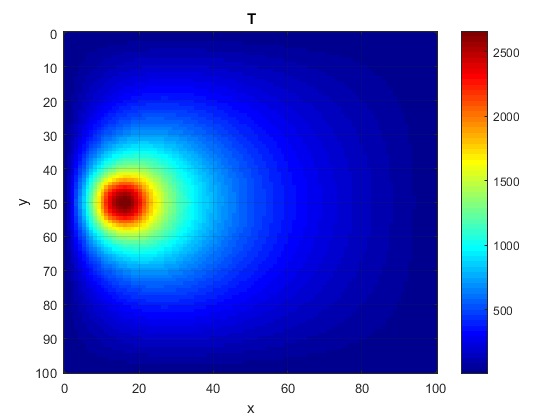
\includegraphics[width=.98\linewidth]{linearT.png}
  \label{fig:sfig1}
\end{subfigure}%
\begin{subfigure}{.5\textwidth}
  \centering
  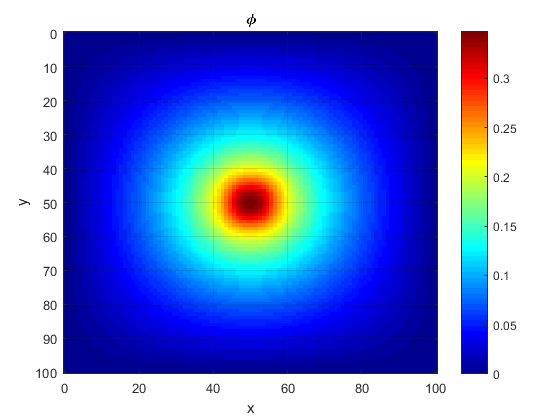
\includegraphics[width=.98\linewidth]{linearphi.png}
  \label{fig:sfig4}
\end{subfigure}%
\caption{Forward and adjoint solutions in MOOSE to linear problem.}
\end{figure}


\begin{table}[H]
\centering
  \begin{tabular}{| l | r | r | r |}
    \hline
    $\delta q$ & $\qoi$ & $\delta \qoi (adj)$ & $\delta \qoi (calc)$ \\ \hline
    $0.02q$ & 6.277803e+02 &  1.055561e+01 & 1.055561e+01  \\ \hline
    $0.04q$ & 6.277803e+02 &  2.111121e+01 & 2.111121e+01 \\ \hline
    $0.06q$ & 6.277803e+02 &  3.166682e+01 & 3.166682e+01  \\ \hline
    $0.08q$ & 6.277803e+02 &  4.222242e+01 & 4.222242e+01  \\ \hline
    $0.10q$ & 6.277803e+02 &  5.277803e+01 & 5.277803e+01  \\ \hline
    \end{tabular}
  \caption{Source perturbation response for linear case. Exact results expected.}
\end{table}

\begin{table}[H]
\centering
  \begin{tabular}{| l | r | r | r |}
    \hline
    $\delta \Tdir$ & $\qoi$ & $\delta \qoi (adj)$ & $\delta \qoi (calc)$ \\ \hline
    $2$ & 6.277803e+02 &  2.000292e+00  &  2.000000e+00   \\ \hline
    $4$ & 6.277803e+02 &  4.000584e+00 &  4.000000e+00  \\ \hline
    $6$ & 6.277803e+02 &  6.000876e+00 &  6.000000e+00   \\ \hline
    $8$ & 6.277803e+02 & 8.001168e+00 & 8.000000e+00   \\ \hline
    $10$ & 6.277803e+02 & 1.000146e+01 & 1.000000e+01   \\ \hline
    \end{tabular}
  \caption{Boundary $\Tdir$ perturbation response for linear case. Exact results expected.}
\end{table}

\begin{table}[H]
\centering
  \begin{tabular}{| l | r | r | r |}
    \hline
    $\delta k$ & $\qoi$ & $\delta \qoi (adj)$ & $\delta \qoi (calc)$ \\ \hline
    $0.02$ & 6.277803e+02 & -8.444485e+00 &   -8.311501e+00  \\ \hline
    $0.04$ & 6.277803e+02 & -1.688897e+01 &  -1.636528e+01  \\ \hline
    $0.06$ & 6.277803e+02 & -2.533345e+01 &   -2.417314e+01  \\ \hline
    $0.08$ & 6.277803e+02 & -3.377794e+01 & -3.174618e+01 \\ \hline
    $0.10$ & 6.277803e+02 & -4.222242e+01 &  -3.909484e+01  \\ \hline
    \end{tabular}
  \caption{Conductivity perturbation response for linear case.}
\end{table}

As expected, the $\delta q$ response is reasonably exact along with $\delta \Tdir$ perturbations, even for large perturbations. There is some slight deviation from the exact observed in the $\Tdir$ when compared to the $q$ perturbations, which was observed in the earlier linear verification problem. The first order nature of the adjoint method begins to appear under $k$ perturbations, even for a linear system. 

\subsection{Non-linear problem}
The next step is to introduce non-linearity into the system.
\begin{equation}
\label{case1}
\begin{split}
& - \div ( k \grad T(\vx) ) = q(\vx) \quad \vx \in \Omega := (0,100) \times (0,100) \\
&T(\vx)=100 \quad \vx \in \partial \Omega \\
& k = 1.05 + \frac{200}{T - 25} \\
& q(\vx) = \left\lbrace 100: x \in (10,20) \times (45,55); \quad 0: \text{ else} \right\rbrace.\\
\end{split}
\end{equation}
The response function is retained from the linear case.

\begin{figure}[H]
\label{sol1}
\centering
\begin{subfigure}{.5\textwidth}
  \centering
  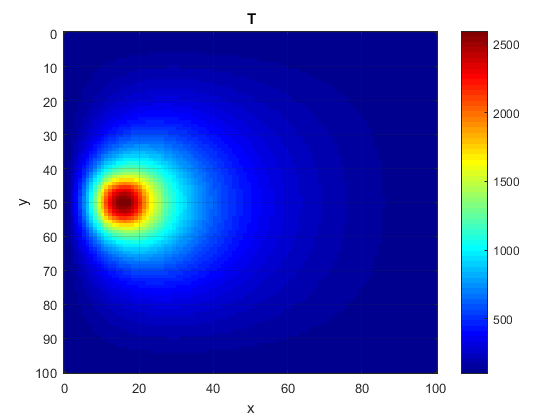
\includegraphics[width=.98\linewidth]{nonlinearT.png}
  \label{fig:sfig1}
\end{subfigure}%
\begin{subfigure}{.5\textwidth}
  \centering
  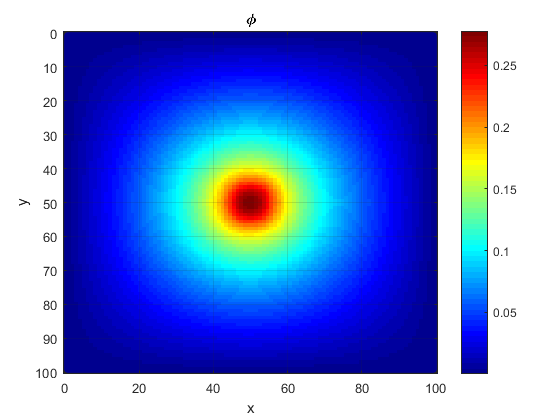
\includegraphics[width=.98\linewidth]{nonlinearphi.png}
  \label{fig:sfig4}
\end{subfigure}%
\caption{Forward and adjoint solutions in MOOSE to nonlinear problem.}
\end{figure}


\begin{table}[H]
\centering
  \begin{tabular}{| l | r | r | r |}
    \hline
    $\delta q$ & $\qoi$ & $\delta \qoi (adj)$ & $\delta \qoi (calc)$ \\ \hline
    $0.02q$ & 4.154273e+02 &  8.456143e+00 & 8.485756e+00  \\ \hline
    $0.04q$ & 4.154273e+02 &  1.691229e+01 & 1.702988e+01 \\ \hline
    $0.06q$ & 4.154273e+02 &  2.536843e+01 & 2.563110e+011  \\ \hline
    $0.08q$ & 4.154273e+02 &  3.382457e+01 & 3.428817e+01  \\ \hline
    $0.10q$ &  4.154273e+02 &   4.228071e+01 & 4.299990e+01  \\ \hline
    \end{tabular}
  \caption{Source perturbation response for nonlinear case.}
\end{table}

\begin{table}[H]
\centering
  \begin{tabular}{| l | r | r | r |}
    \hline
    $\delta \Tdir$ & $\qoi$ & $\delta \qoi (adj)$ & $\delta \qoi (calc)$ \\ \hline
    $2$ & 4.154273e+02  &  4.744641e+00  &  4.707770e+00    \\ \hline
    $4$ & 4.154273e+02  &  9.489283e+00 &  9.347356e+00 \\ \hline
    $6$ & 4.154273e+02  &  1.423392e+01 &  1.392190e+01   \\ \hline
    $8$ & 4.154273e+02  &  1.897857e+01 & 1.843434e+01  \\ \hline
    $10$ & 4.154273e+02  & 2.372321e+01 & 2.288741e+01   \\ \hline
    \end{tabular}
  \caption{Boundary $\Tdir$ perturbation response for nonlinear case.}
\end{table}

\begin{table}[H]
\centering
  \begin{tabular}{| l | r | r | r |}
    \hline
    $\delta k$ & $\qoi$ & $\delta \qoi (adj)$ & $\delta \qoi (calc)$ \\ \hline
    $0.02$ & 4.154273e+02 & -4.048877e+00 &  -3.990900e+00  \\ \hline
    $0.04$ & 4.154273e+02 & -8.097754e+00 &  -7.869313e+00  \\ \hline
    $0.06$ & 4.154273e+02 & -1.214663e+01 &  -1.164020e+01  \\ \hline
    $0.08$ & 4.154273e+02  &  -1.619551e+01 & -1.530823e+01 \\ \hline
    $0.10$ &  4.154273e+02 &  -2.024439e+01 & -1.887780e+01  \\ \hline
    \end{tabular}
  \caption{Conductivity perturbation response for nonlinear case.}
\end{table}

As non-linearity is introduced to the system, more first order approximation mus the made, so the exact nature of the source perturbation is lost. Even then, the method appears to make a reasonable (within 10\% of the true $\delta \qoi$) approximation of the response to perturbations.

\subsection{``Heater'' problem }
We now introduce a bit more of a complex source configuration, where the detector is located between two heating bars. This should yield a more interesting temperature profile.
\begin{equation}
\label{case3}
\begin{split}
& - \div ( k \grad T(\vx) ) = q(\vx) \quad \vx \in \Omega := (0,100) \times (0,100) \\
&T(\vx)=10 \quad \vx \in \partial \Omega \\
& k = 1.05 + \frac{200}{T - 25} \\
& q(\vx) = \left\lbrace 100: x \in [(20,80) \times (20,30) \cup (20,80) \times (70,80) ]; \quad 0: \text{ else} \right\rbrace.\\
\end{split}
\end{equation}
The response function remains unchanged.

\begin{figure}[H]
\label{sol1}
\centering
\begin{subfigure}{.5\textwidth}
  \centering
  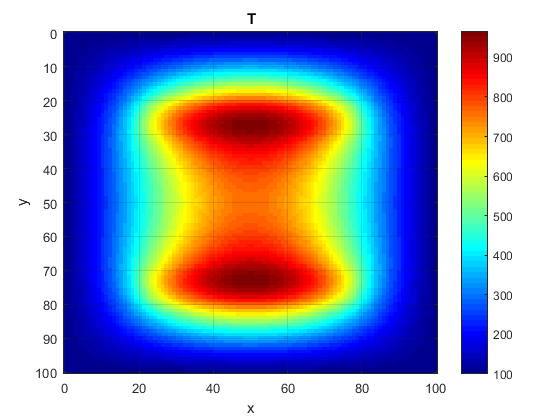
\includegraphics[width=.98\linewidth]{nonlinear2T.png}
  \label{fig:sfig1}
\end{subfigure}%
\begin{subfigure}{.5\textwidth}
  \centering
  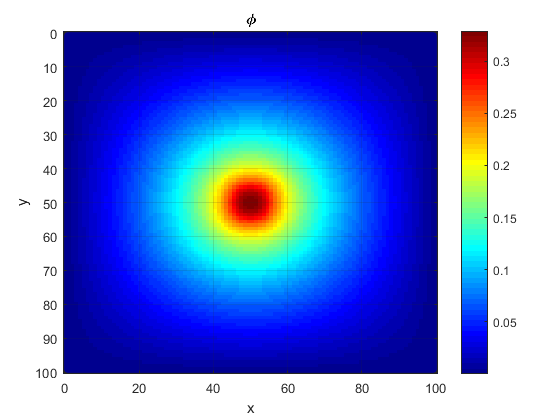
\includegraphics[width=.98\linewidth]{nonlinear2phi.png}
  \label{fig:sfig4}
\end{subfigure}%
\caption{Forward and adjoint solutions in MOOSE to linear problem.}
\end{figure}


\begin{table}[H]
\centering
  \begin{tabular}{| l | r | r | r |}
    \hline
    $\delta q$ & $\qoi$ & $\delta \qoi (adj)$ & $\delta \qoi (calc)$ \\ \hline
    $0.02q$ & 7.604237e+02 &   1.739914e+01 & 1.744103e+01  \\ \hline
    $0.04q$ & 7.604237e+02 &  3.479828e+01 & 3.496404e+01 \\ \hline
    $0.06q$ & 7.604237e+02 &  5.219742e+01 & 5.256644e+01  \\ \hline
    $0.08q$ & 7.604237e+02 &  6.959656e+01 & 7.024574e+01  \\ \hline
    $0.10q$ & 7.604237e+02 &  8.699570e+01 & 8.799956e+01  \\ \hline
    \end{tabular}
  \caption{Source perturbation response for heater case.}
\end{table}

\begin{table}[H]
\centering
  \begin{tabular}{| l | r | r | r |}
    \hline
    $\delta \Tdir$ & $\qoi$ & $\delta \qoi (adj)$ & $\delta \qoi (calc)$ \\ \hline
    $2$ & 7.604237e+02 &  5.624113e+00  &  5.574747e+00   \\ \hline
    $4$ & 7.604237e+02 &  1.124823e+01 &  1.105566e+01   \\ \hline
    $6$ & 7.604237e+02 &  1.687234e+01 &  1.644732e+01   \\ \hline
    $8q$ & 7.604237e+02 & 2.249645e+01 & 2.175398e+01   \\ \hline
    $10$ & 7.604237e+02 & 2.812057e+01  & 2.697960e+01   \\ \hline
    \end{tabular}
  \caption{Boundary $\Tdir$ perturbation response for heater case.}
\end{table}

\begin{table}[H]
\centering
  \begin{tabular}{| l | r | r | r |}
    \hline
    $\delta k$ & $\qoi$ & $\delta \qoi (adj)$ & $\delta \qoi (calc)$ \\ \hline
    $0.02$ & 7.604237e+02 & -9.991441e+00 &  -9.829103e+00  \\ \hline
    $0.04$ & 7.604237e+02 & -1.998288e+01 &  -1.934429e+01  \\ \hline
    $0.06$ & 7.604237e+02 & -2.997432e+01 &  -2.856091e+01  \\ \hline
    $0.08$ & 7.604237e+02 & -3.996576e+01 &  -3.749328e+01 \\ \hline
    $0.10$ & 7.604237e+02 & -4.995720e+01 &  -4.615482e+01  \\ \hline
    \end{tabular}
  \caption{Conductivity perturbation response for heater case.}
\end{table}
This nonlinear heater scenario continues to follow the trend set by the previous nonlinear test case, where the approximation via adjoint appears to be reasonable. 

\begin{thebibliography}{9}
\bibitem{MOOSE}
Gaston, Derek, et al. \textit{MOOSE: A parallel computational framework for coupled systems of nonlinear equations.}
 Nuclear Engineering and Design 239.10 (2009): 1768-1778.
 
\bibitem{Marchuk}
G. I. Marchuk \textit{Adjoint Equations and Analysis of Complex Systems.}
Springer, 1995.
\end{thebibliography}

\end{document}